To verify that the our measured HRTFs are free of artifacts (e.g., pre-responses prior to the main impulses), we generate a surface plot of ITD estimated from measured HRTFs using a thresholding approach (see, for example, \citet{KatzNoisternig2014}) with a 20\% threshold.
\Figref{fig:Sample_ITD_surface} shows this surface plot for one of the subjects in our database.
This plot shows a plausible ITD surface, as it is generally smooth and free of discontinuities, suggesting that the data are free of significant artifacts, noise, or any other errors.

\begin{figure}[t]
\begin{center}
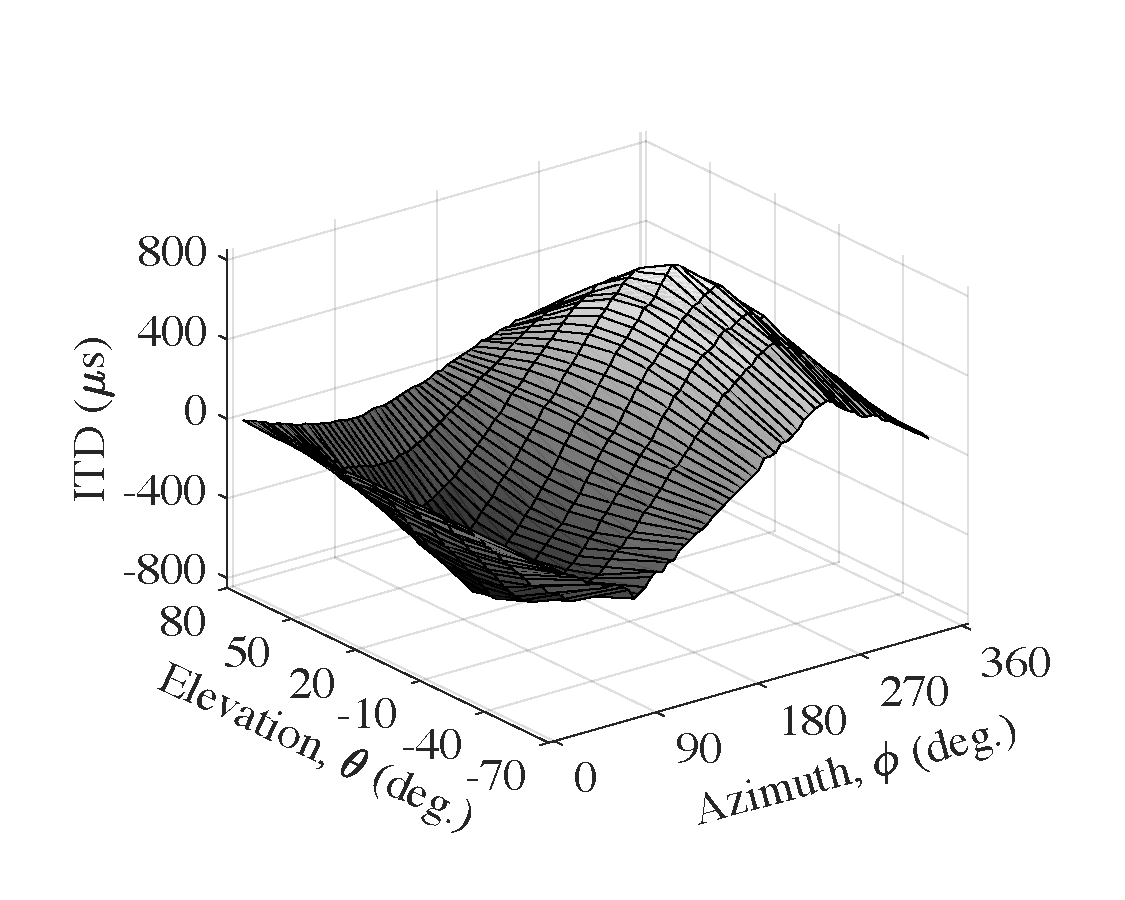
\includegraphics[width = 0.7\textwidth]{a4_HRTF_measurements/figures/Sample_ITD_surface.pdf}
\caption[Surface plot of typical interaural time differences.]{Surface plot of ITD in $\mu s$ for one of the subjects in our database.}.
\label{fig:Sample_ITD_surface}
\end{center}
\end{figure}